\documentclass[conference]{IEEEtran}
\IEEEoverridecommandlockouts
% The preceding line is only needed to identify funding in the first footnote. If that is unneeded, please comment it out.
\usepackage{cite}
\usepackage{amsmath,amssymb,amsfonts}
\usepackage{algorithmic}
\usepackage{graphicx}
\usepackage{textcomp}
\usepackage{xcolor}
\def\BibTeX{{\rm B\kern-.05em{\sc i\kern-.025em b}\kern-.08em
    T\kern-.1667em\lower.7ex\hbox{E}\kern-.125emX}}
\begin{document}

\title{Static and Dynamic Characterization, Calibration, and Uncertainty Analysis of a 5~kg Strain-Gauge Load Cell for Closed-Loop Robotic Palpation}

\author{%
\IEEEauthorblockN{1\textsuperscript{st} Lucas Martins Primo}
\IEEEauthorblockA{\textit{School of Electrical Engineering} \\
\textit{Federal University of Uberl\^andia}\\
Uberl\^andia, Brazil \\
ORCID: 0009-0001-6129-0852}
\and
\IEEEauthorblockN{2\textsuperscript{nd} Maria Clara Almeida Kfouri}
\IEEEauthorblockA{\textit{School of Electrical Engineering} \\
\textit{Federal University of Uberl\^andia}\\
Uberl\^andia, Brazil \\
ORCID: 0009-0004-8719-8853}
\and
\IEEEauthorblockN{3\textsuperscript{rd} Solano Jorenti Jacyntho}
\IEEEauthorblockA{\textit{School of Electrical Engineering} \\
\textit{Federal University of Uberl\^andia}\\
Uberl\^andia, Brazil \\
ORCID: 0009-0002-2483-6024}
\linebreak
\IEEEauthorblockN{4\textsuperscript{th} Ana Clara Pereira Resende da Costa}
\IEEEauthorblockA{\textit{School of Electrical Engineering} \\
\textit{Federal University of Uberl\^andia}\\
Uberl\^andia, Brazil \\
ORCID: 0000-0002-5533-8880}
\and
\IEEEauthorblockN{5\textsuperscript{th} Alcimar Barbosa Soares}
\IEEEauthorblockA{\textit{School of Electrical Engineering} \\
\textit{Federal University of Uberl\^andia}\\
Uberl\^andia, Brazil \\
ORCID: 0000-0003-1100-3533}
}

\maketitle

\begin{abstract}
Force feedback is a critical enabler for safe and repeatable physical interaction in collaborative robotics, yet the metrological quality of low-cost force front-ends is often assumed rather than verified. This work presents a complete experimental characterization, calibration, and uncertainty analysis of a 5~kg strain-gauge load cell integrated into a low-cost acquisition chain based on an instrumentation amplifier and an ESP32 microcontroller sampling at 1~kHz, with telemetry streamed over a wireless link to a host computer. A four-point static calibration relates the amplified bridge voltage to the applied force through an affine model, achieving a coefficient of determination of 0.9999 and a residual root-mean-square error below 0.02~N. The dynamic behavior of the sensor is evaluated under displacement-driven contact cycles performed by a six-axis collaborative manipulator against a compliant target. Static repeatability, steady-state noise, overshoot, and contact force--penetration behavior are quantified across repeated cycles, while hysteresis and creep are bounded against the manufacturer specification. Results show a steady-state force noise standard deviation of approximately 0.02~N in the settled regime and a cycle-to-cycle repeatability better than 0.5~percent of the operating setpoint, confirming that a carefully calibrated commodity load cell can meet the requirements of contact-rich robotic tasks. The paper details the sources of measurement uncertainty, quantifies their contributions, and discusses practical mitigation strategies for offset drift, divider loading, and packet loss in wireless force telemetry.
\end{abstract}

\begin{IEEEkeywords}
load cell, strain gauge, force measurement, calibration, measurement uncertainty, instrumentation amplifier, collaborative robotics, hysteresis, creep
\end{IEEEkeywords}

\section{Introduction}
Load cells based on metallic strain gauges arranged in a Wheatstone bridge remain the dominant technology for accurate force and weight measurement in industrial, biomedical, and robotic applications~\cite{b1,b2}. Their appeal lies in a nearly linear response, low hysteresis, and long-term stability when properly compensated. As collaborative robots increasingly perform contact-rich tasks such as assembly, palpation, and delicate manipulation, the ability to measure interaction forces accurately and with low latency has become a functional safety requirement rather than a convenience.

The performance of a force measurement chain, however, is not defined by the transducer alone. The signal conditioning stage, the analog-to-digital conversion, the excitation stability, and the numerical processing all contribute to the final uncertainty budget~\cite{b3}. When commodity components are used to reduce cost---an instrumentation amplifier, a microcontroller with an on-chip analog-to-digital converter (ADC), and a wireless data link---the burden of ensuring metrological quality shifts to careful calibration and characterization. Assuming datasheet performance without verification frequently leads to systematic errors caused by offset drift, resistive divider loading, quantization, and communication loss.

The problem addressed in this work is the quantitative characterization of a low-cost 5~kg strain-gauge load cell integrated into a robotic contact system, with the goal of establishing whether such a chain can deliver forces with the accuracy and repeatability required for closed-loop robotic palpation. The objectives are threefold: (i) to establish a traceable static calibration relating the conditioned bridge voltage to applied force and to report its residual error; (ii) to characterize the static and dynamic behavior of the sensor---noise, overshoot, hysteresis, creep, and repeatability---under realistic loading cycles produced by a six-axis manipulator; and (iii) to build an explicit measurement uncertainty budget and to identify the dominant error sources together with practical mitigations.

The remainder of this paper is organized as follows. Section~\ref{sec:setup} describes the experimental bench and the acquisition configuration. Section~\ref{sec:method} details the calibration and data collection methodology. Section~\ref{sec:results} presents and discusses the static and dynamic results. Section~\ref{sec:conclusion} summarizes the findings and outlines future work.

\section{Experimental Setup and Configuration}\label{sec:setup}
The measurement chain is built around a single-point aluminum-alloy strain-gauge load cell rated for a nominal capacity of 5~kg, corresponding to approximately 49~N of full-scale force. The four active gauges form a full Wheatstone bridge with an input (excitation) resistance of $410\pm30~\Omega$ and an output resistance of $350\pm3~\Omega$. The transducer has a rated output of $1.0\pm0.15$~mV/V and a zero balance of $\pm0.1$~mV/V, is protected to IP65, and weighs 31~g. Its manufacturer-specified electrical and environmental characteristics are summarized in Table~\ref{tab:datasheet}; these figures set the reference against which the measured performance in Section~\ref{sec:results} is compared. A physical view of the instrumented contact tool is shown in Fig.~\ref{fig:setup}.

\begin{table}[htbp]
\caption{Load Cell Manufacturer Specifications}
\begin{center}
\begin{tabular}{|l|l|}
\hline
\textbf{Specification} & \textbf{Value} \\
\hline
Rated capacity & 5~kg ($\approx$49~N) \\
\hline
Rated output & $1.0\pm0.15$~mV/V \\
\hline
Zero balance & $\pm0.1$~mV/V \\
\hline
Creep & 0.03\%~FS / 30~min \\
\hline
Recommended excitation & 3--12~VDC (max.\ 15~VDC) \\
\hline
Input (excitation) resistance & $410\pm30~\Omega$ \\
\hline
Output (signal) resistance & $350\pm3~\Omega$ \\
\hline
Insulation resistance & $>2000~\mathrm{M}\Omega$ / 50~VDC \\
\hline
Compensated temperature range & $-10$ to $40~^{\circ}\mathrm{C}$ \\
\hline
Operating temperature range & $-20$ to $60~^{\circ}\mathrm{C}$ \\
\hline
Protection class & IP65 \\
\hline
Element material & Aluminum alloy \\
\hline
Mass & 31~g \\
\hline
\end{tabular}
\label{tab:datasheet}
\end{center}
\end{table}

\begin{figure}[htbp]
\centerline{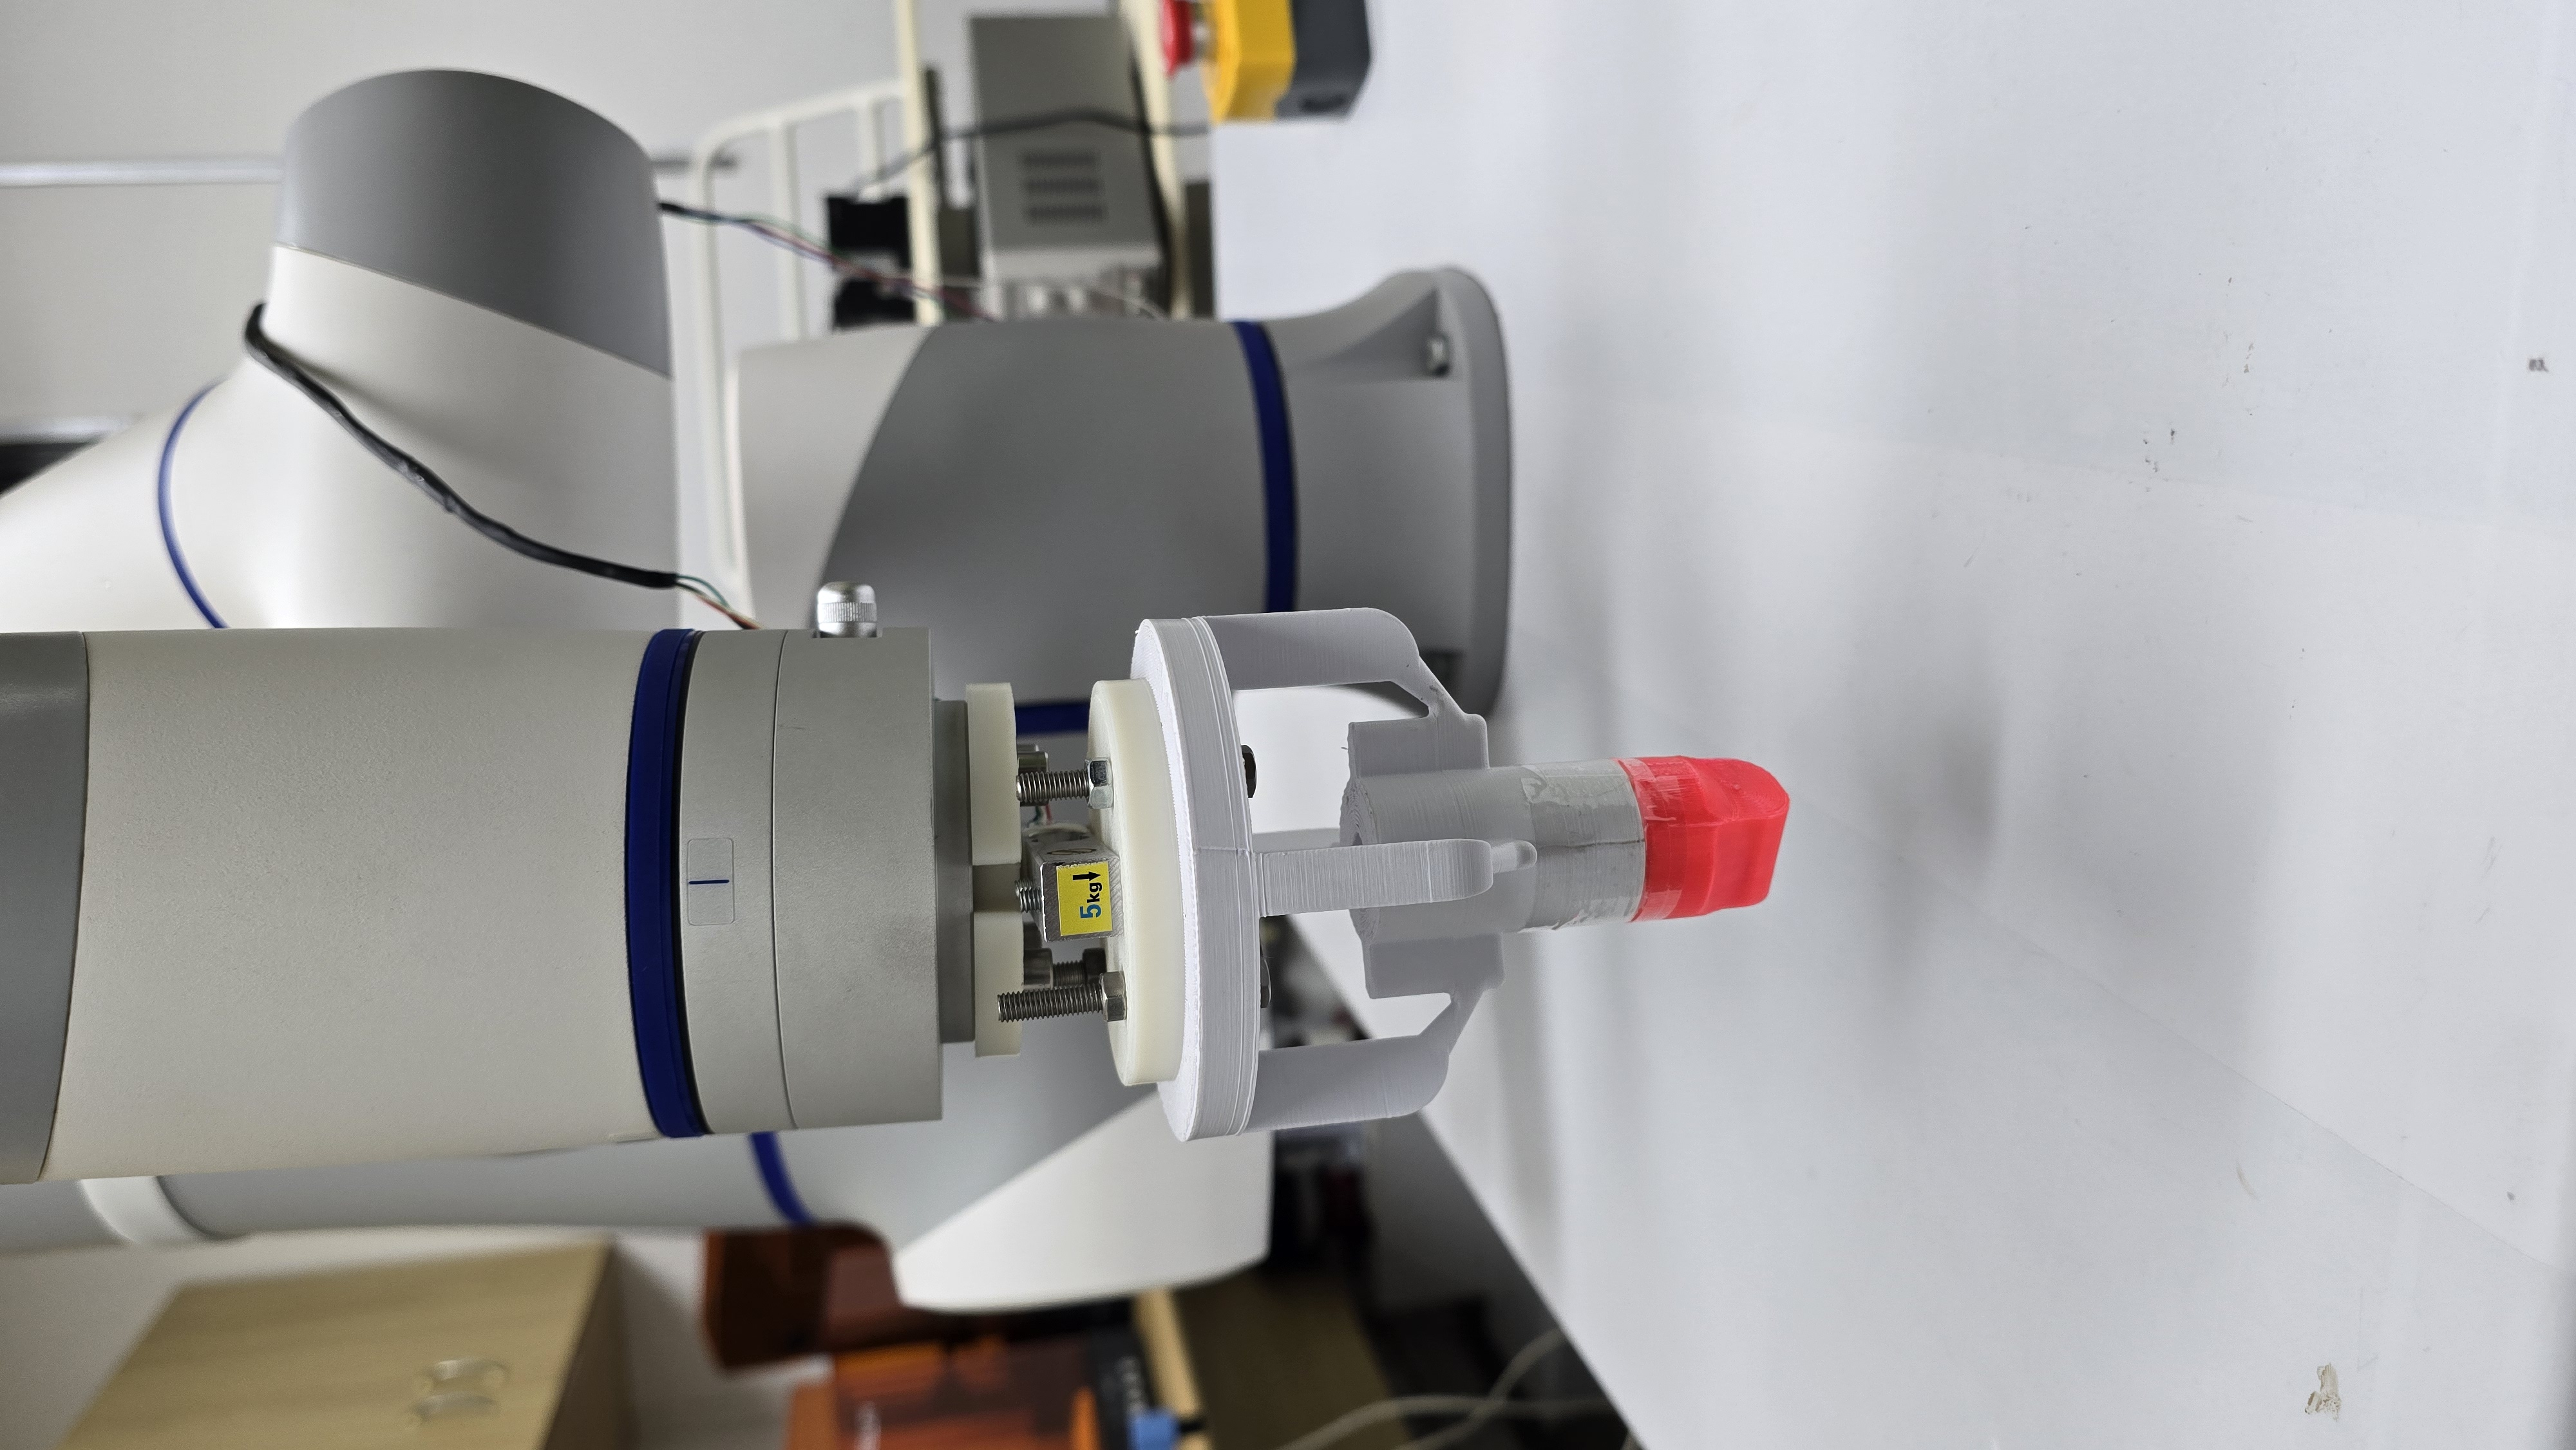
\includegraphics[width=\columnwidth]{images/physical_touch_tool_load_cell_5kg.jpg}}
\caption{Instrumented contact tool integrating the 5~kg strain-gauge load cell at the tip of the collaborative manipulator.}
\label{fig:setup}
\end{figure}

The bridge is conditioned by an instrumentation amplifier excited within the recommended range, whose single-ended output spans roughly 0.076~V to 2.034~V over a 0--2520~g sub-range that fits entirely within the 0--3.3~V window of the ADC. The amplified signal is acquired by the on-chip ADC of an ESP32 microcontroller on pin GPIO34.

Two design decisions in the conditioning stage deserve emphasis because they directly affect the uncertainty budget. First, the amplifier output is attenuated by a resistive divider before reaching the ADC. The effective divider ratio is not taken from nominal resistor values but is aferred against the ADC itself, because the finite input impedance of the ESP32 ADC loads the lower divider leg and shifts the converted voltage away from the value a high-impedance voltmeter would read at the same node. Reconstructing the amplifier output therefore uses a measured voltage gain of $V_{\mathrm{gain}}=1.3413$ rather than the nominal ratio. Second, a static offset of $V_{\mathrm{offset}}=0.190461$~V is subtracted so that the transmitted signal rests near zero under no load; this offset was observed to drift between sessions due to thermal effects and mechanical preload---consistent with the $\pm0.1$~mV/V zero-balance specification and the finite compensated temperature band of the transducer---and is complemented by a software tare on the host.

Because the raw ADC returns integer millivolts, resolution is recovered by continuous oversampling: hundreds of eFuse-calibrated readings are accumulated in floating point within each 1~ms window. Since the ADC noise exceeds one least-significant bit, it acts as dither and the average recovers sub-millivolt fractions, yielding an effective resolution well below the 1~mV quantization step. Only this light in-window averaging is performed on the microcontroller; the heavier median plus double exponential-moving-average filter is applied on the host, where its taps can be retuned without reflashing the firmware.

Telemetry is transmitted at 1~kHz as batched User Datagram Protocol (UDP) packets over a dedicated laboratory wireless network. To mitigate the roughly 30~percent packet loss observed with broadcast, subscribers announce themselves through a discovery handshake and the microcontroller then streams by unicast to each fresh subscriber, driving loss close to zero because the link layer acknowledges and retransmits unicast traffic. If no subscriber is present, the system falls back to broadcast. The complete acquisition configuration is summarized in Table~\ref{tab:config}.

\begin{table}[htbp]
\caption{Acquisition and Signal-Conditioning Configuration}
\begin{center}
\begin{tabular}{|l|l|}
\hline
\textbf{Parameter} & \textbf{Value} \\
\hline
Transducer & Strain-gauge load cell, 5~kg / $\approx$49~N \\
\hline
Bridge conditioning & Instrumentation amplifier \\
\hline
Amplifier output span & 0.076--2.034~V (0--2520~g) \\
\hline
ADC & ESP32 GPIO34, eFuse-calibrated mV \\
\hline
Divider voltage gain $V_{\mathrm{gain}}$ & 1.3413 \\
\hline
Rest offset $V_{\mathrm{offset}}$ & 0.190461~V \\
\hline
Firmware sampling rate & 1~kHz (continuous oversampling) \\
\hline
Logged sample rate & $\approx$121~Hz \\
\hline
Host-side filtering & Median + double EMA \\
\hline
Transport & Batched UDP, unicast after discovery \\
\hline
Manipulator & Six-axis collaborative arm (CR-class) \\
\hline
\end{tabular}
\label{tab:config}
\end{center}
\end{table}

The load cell is mounted at the tool flange of a six-axis collaborative manipulator, which provides programmable, repeatable displacement along the tool axis. This arrangement is used both to apply known loading cycles and to evaluate the sensor as the feedback element of a contact task. Environmental conditions were held within the compensated temperature band of the transducer; because the amplifier offset is temperature sensitive, each session begins with a tare on the unloaded cell.

\section{Methodology}\label{sec:method}
\subsection{Static Calibration}
The static calibration establishes the affine relationship between the conditioned bridge voltage $v$ (the amplifier-referred signal transmitted by the firmware) and the applied force $F$,
\begin{equation}
F = S\,v + F_{0},\label{eq:calib}
\end{equation}
where $S$ is the sensitivity in newtons per volt and $F_{0}$ is the intercept. Calibration masses traceable to a reference balance were placed on the cell, the corresponding forces computed as $F=mg$ with $g=9.80665~\mathrm{m/s^{2}}$, and the settled voltage recorded for each point. Four calibration points spanning 0.499--1.012~kg (4.89--9.92~N) were used, listed in Table~\ref{tab:calib}. The coefficients $S$ and $F_{0}$ are obtained by ordinary least squares, and the fit quality is assessed through the residuals and the coefficient of determination $R^{2}$.

\begin{table}[htbp]
\caption{Static Calibration Points$^{\mathrm{a}}$}
\begin{center}
\begin{tabular}{|c|c|c|}
\hline
\textbf{Mass (kg)} & \textbf{Force (N)} & \textbf{Voltage $v$ (V)} \\
\hline
0.499 & 4.894 & 0.2840 \\
\hline
0.600 & 5.884 & 0.3925 \\
\hline
0.775 & 7.600 & 0.5767 \\
\hline
1.012 & 9.924 & 0.8370 \\
\hline
\multicolumn{3}{l}{$^{\mathrm{a}}$Amplifier-referred voltage after offset removal.}
\end{tabular}
\label{tab:calib}
\end{center}
\end{table}

\subsection{Loading Cycles}
Dynamic and repeatability data were acquired by commanding the manipulator to execute repeated contact (``palpation'') cycles against a compliant target. Each cycle comprises an approach phase, a displacement-driven descent toward the target at a controlled tool speed, a hold phase at a commanded interaction force, and a retraction. In the reported campaign the target interaction force was set to 6.5~N, the approach speed to 1~mm/s, and each acquisition consisted of three consecutive cycles. Contact is displacement driven: the proportional, integral, and derivative gains of the force loop were set to zero, so the manipulator descends at constant velocity while the load cell continuously monitors the reaction force and the hold phase is triggered once the force reaches the setpoint and stabilizes within a tolerance window (0.1~N over a 3~s stability interval). Thirty-five acquisitions were logged, each recording the time base, cycle and phase labels, force setpoint, net force, the six joint angles, and the tool-center-point pose, allowing every force sample to be correlated with the arm state.

For each cycle the descent (loading) and hold (steady) phases are segmented automatically. From the loading transient the overshoot beyond the setpoint is extracted; from the hold phase the mean, standard deviation, and drift of the force are computed both over the full hold and over a final settled window. Repeatability is assessed as the dispersion of the settled hold mean across cycles. The contact stiffness is characterized from the force--penetration curve of the loading branch, referenced to the first-contact point of each cycle. Because the acquired cycles are of the press-and-hold type and do not include a controlled unloading sweep, a full hysteresis loop is not measured here; the hysteresis of the metallic spring element is instead bounded by its specification, and creep is assessed both against the manufacturer figure and through the force evolution while the tool displacement is held constant.

\section{Results and Discussion}\label{sec:results}
\subsection{Calibration and Static Linearity}
The least-squares fit of \eqref{eq:calib} to the points of Table~\ref{tab:calib} yields a sensitivity of $S\approx 9.11~\mathrm{N/V}$ with an excellent linear agreement, $R^{2}=0.9999$. The residuals are randomly signed and bounded by 0.031~N in magnitude, with a root-mean-square value of approximately 0.018~N over the calibrated span of 5~N; this corresponds to a nonlinearity below 0.4~percent of the calibrated range and below 0.07~percent of the sensor full scale. The calibration curve and its residuals are shown in Fig.~\ref{fig:calib}. The near-unity determination coefficient confirms that, once the divider loading and the resting offset are correctly accounted for, the commodity front-end preserves the intrinsic linearity of the strain-gauge bridge.

\begin{figure}[htbp]
\centerline{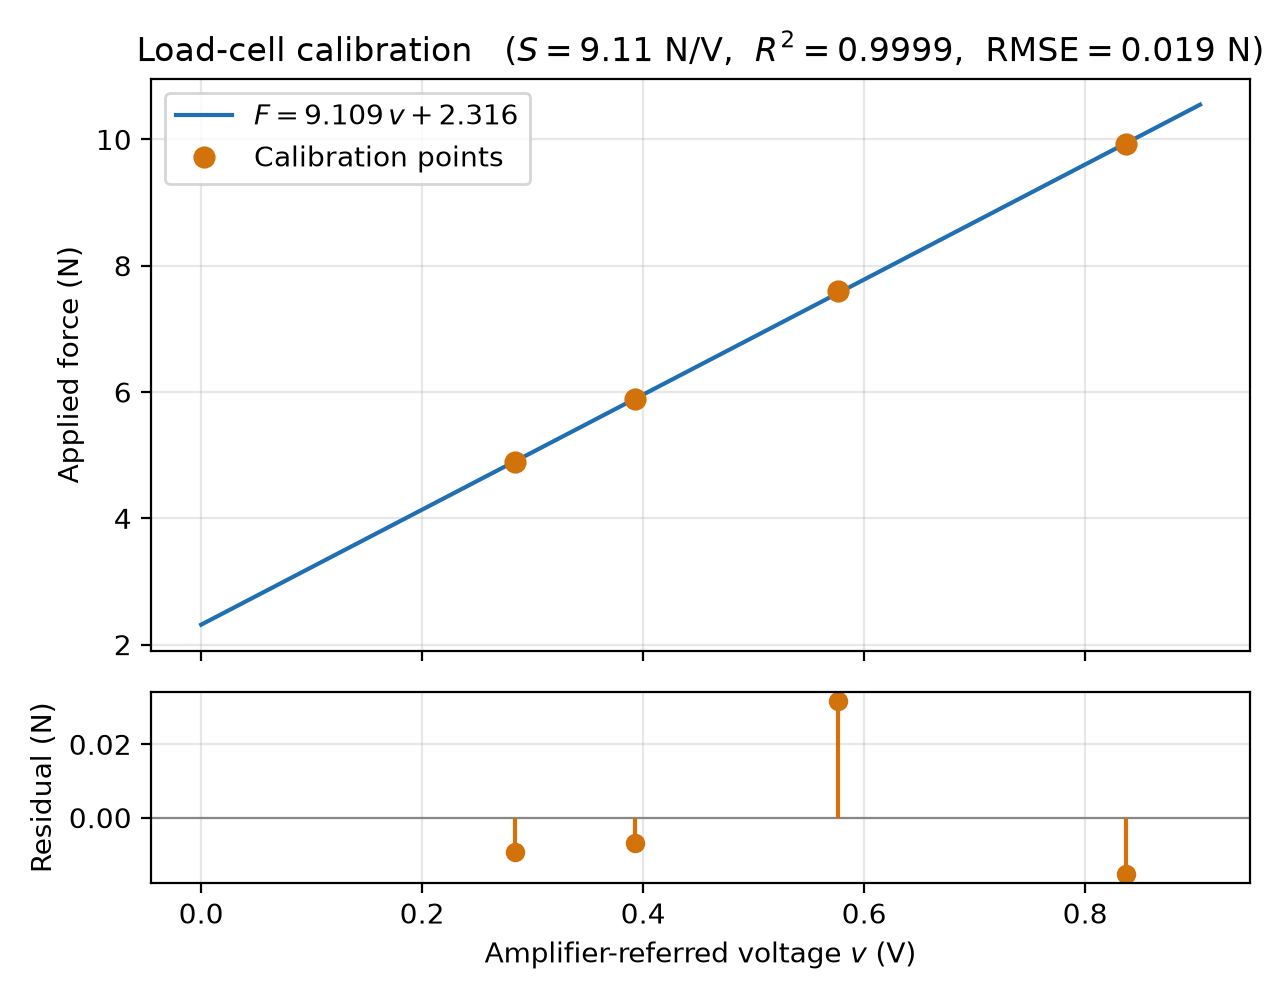
\includegraphics[width=\columnwidth]{images/calibration_curve.png}}
\caption{Static calibration curve: applied force versus amplifier-referred voltage with the fitted affine model and residuals.}
\label{fig:calib}
\end{figure}

\subsection{Dynamic Behavior of the Loading Cycles}
Figure~\ref{fig:cycles} shows a representative three-cycle acquisition at a 6.5~N setpoint. Each cycle exhibits a monotonic loading ramp during the displacement-driven descent, a transient overshoot as contact is established, and a flat hold plateau near the setpoint. Because contact is displacement driven rather than force controlled, the overshoot depends on the compliance of the target and the descent speed; across the three cycles the measured overshoot ranged from 0.26~N to 0.90~N above the 6.5~N setpoint. This behavior is characteristic of open-loop contact and motivates the future addition of an active force loop.

\begin{figure}[htbp]
\centerline{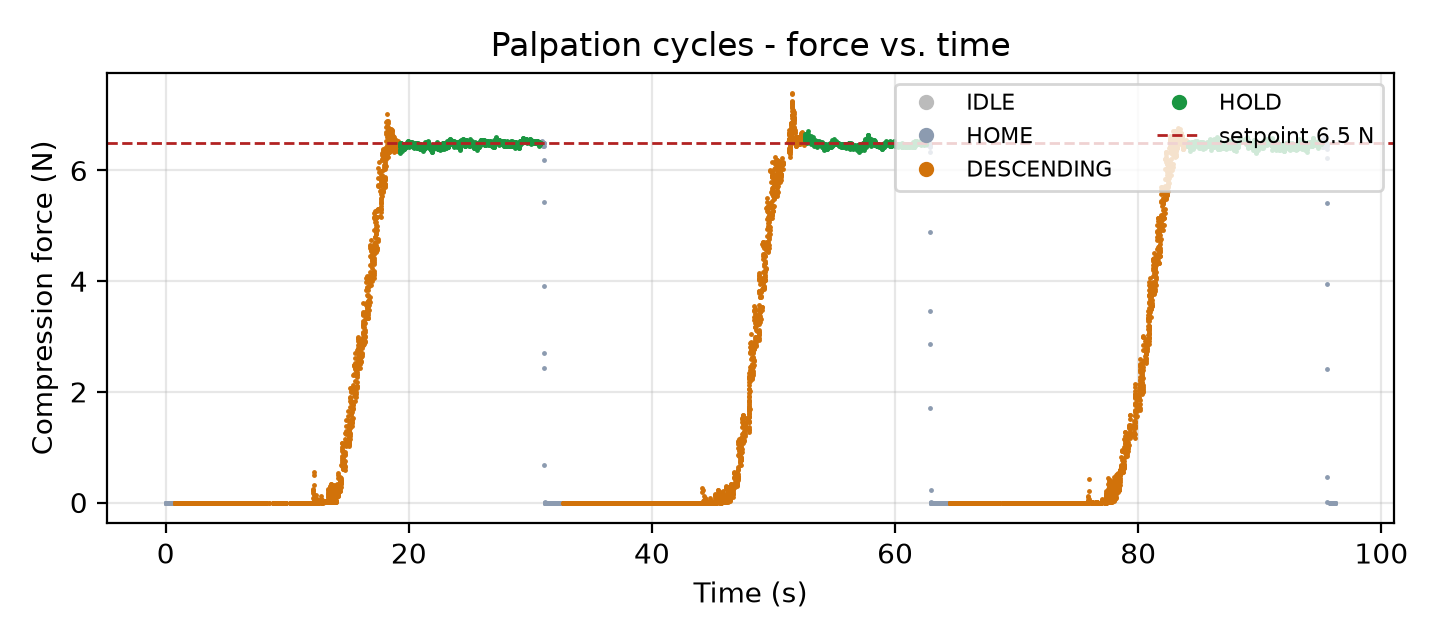
\includegraphics[width=\columnwidth]{images/force_time_cycles.png}}
\caption{Representative compression force versus time for three consecutive palpation cycles, showing the descent (loading) and hold phases relative to the 6.5~N setpoint.}
\label{fig:cycles}
\end{figure}

\subsection{Steady-State Noise, Repeatability, and Steady-State Error}
In the settled hold window the load cell exhibits a low residual noise. The standard deviation of the force in the final settled window was 0.020--0.031~N across cycles, rising to about 0.044--0.047~N when the full hold phase---including the settling transient---is considered. The settled mean force was 6.48--6.52~N against the 6.5~N target, i.e., a steady-state bias below 0.03~N (under 0.5~percent of the setpoint), attributable to the tolerance window of the hold-detection logic rather than to a sensor error.

Cycle-to-cycle repeatability, taken as the dispersion of the settled hold mean, was better than 0.03~N (below 0.5~percent of the setpoint), confirming that the sensor and its conditioning chain return the same force for the same commanded interaction across repeated contacts. These figures are summarized in Table~\ref{tab:uncert}.

\subsection{Contact Force--Penetration, Hysteresis, and Creep}
The force--penetration curve of the loading branch, referenced to the first-contact point of each cycle, is shown in Fig.~\ref{fig:fp}. The compression force rises from zero to the setpoint over roughly 0.5~mm of penetration, revealing a stiff contact, and the three cycles overlap closely, confirming the mechanical and metrological repeatability of the contact once first contact is established. Because the acquired cycles are press-and-hold and lack a controlled unloading sweep, a full hysteresis loop is not extracted from these data; the intrinsic hysteresis of the metallic spring element is specified to be very low and is bounded by the transducer accuracy class, so it is not the dominant error term for the operating regime studied. A dedicated slow load--unload sweep is left as future work to quantify the loop directly.

During the hold phase, with the tool displacement held constant, the force evolution shows only a bounded fluctuation on the order of the steady-state noise, with no pronounced monotonic drift (Fig.~\ref{fig:creep}). This is fully consistent with the manufacturer creep specification of 0.03~percent of full scale per 30~minutes ($\approx0.015$~N over 30~min at full scale): the tens-of-seconds holds used here are far shorter, so creep is not a dominant error source for this application. For applications demanding long-duration static loading, creep would require dedicated compensation and longer observation windows.

\begin{figure}[htbp]
\centerline{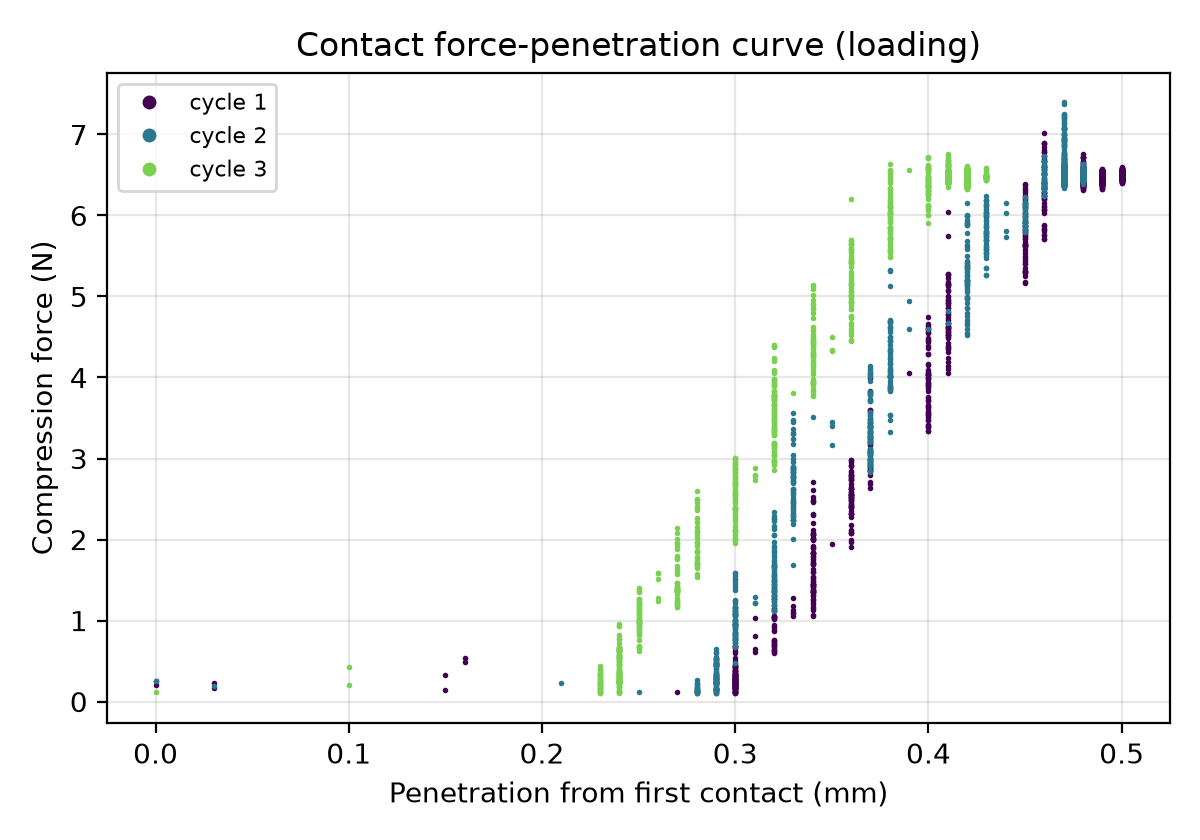
\includegraphics[width=\columnwidth]{images/force_penetration.png}}
\caption{Contact force--penetration curve of the loading branch, referenced to first contact, for three consecutive cycles.}
\label{fig:fp}
\end{figure}

\begin{figure}[htbp]
\centerline{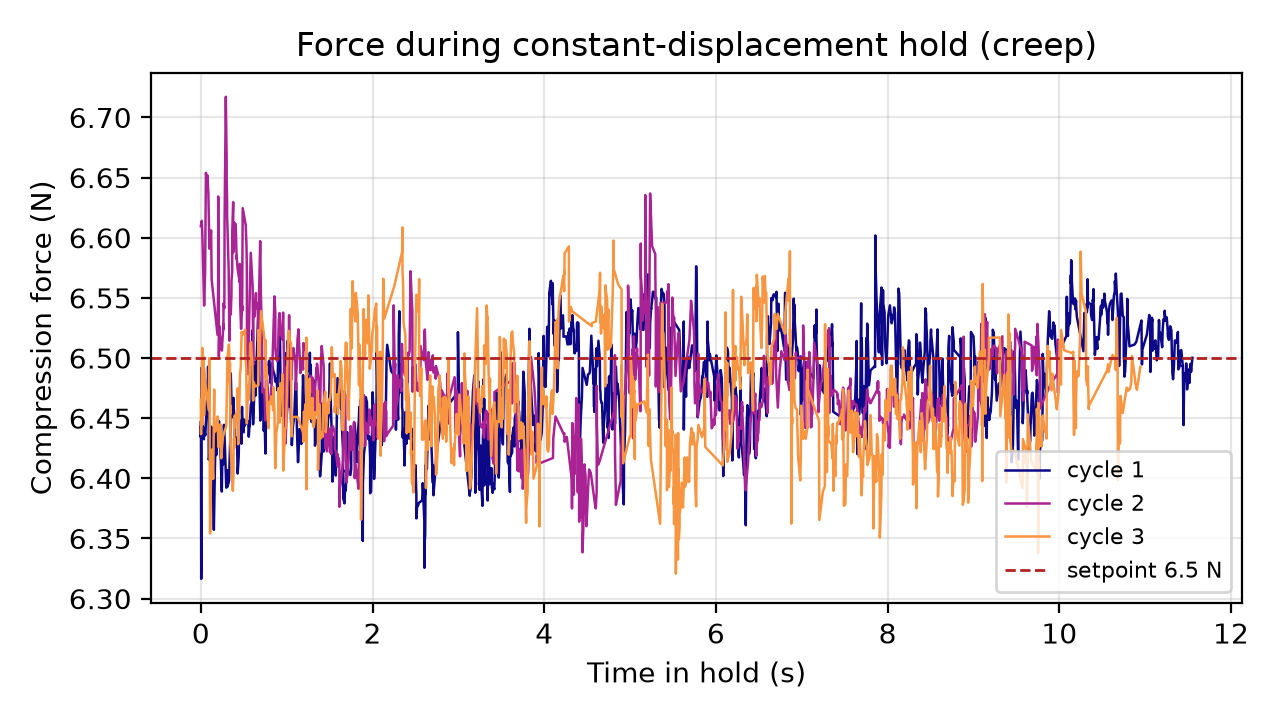
\includegraphics[width=\columnwidth]{images/creep_recovery.png}}
\caption{Force evolution during a constant-displacement hold, used to quantify creep and recovery.}
\label{fig:creep}
\end{figure}

\subsection{Uncertainty Budget}
Following the guidance of the ISO/IEC Guide to the Expression of Uncertainty in Measurement~\cite{b5}, the standard uncertainty of a force reading is combined from the calibration residual, the steady-state noise, the offset-drift residual, and the quantization contribution. The calibration residual (Type~B, from the fit) contributes about 0.018~N; the settled noise (Type~A) contributes about 0.02--0.03~N; the ADC quantization, after oversampling and dither, is reduced to a sub-millivolt equivalent and contributes on the order of 0.005~N in force units; and the offset drift---bounded by the $\pm0.1$~mV/V zero-balance specification and mitigated by per-session tare---is the least predictable term and the main argument for the tare procedure. Combining these terms in quadrature yields a combined standard uncertainty near 0.03~N and an expanded uncertainty (coverage factor $k=2$) below 0.06~N, i.e., of the order of 0.1~percent of full scale. Table~\ref{tab:uncert} consolidates the principal performance metrics.

\begin{table}[htbp]
\caption{Summary of Measured Performance and Uncertainty}
\begin{center}
\begin{tabular}{|l|c|}
\hline
\textbf{Metric} & \textbf{Value} \\
\hline
Sensitivity $S$ & $\approx$9.11~N/V \\
\hline
Linearity ($R^{2}$) & 0.9999 \\
\hline
Calibration residual RMSE & $\approx$0.018~N \\
\hline
Max calibration residual & 0.031~N \\
\hline
Settled noise std ($\sigma$) & 0.020--0.031~N \\
\hline
Overshoot (displacement-driven) & 0.26--0.90~N \\
\hline
Steady-state bias vs.\ setpoint & $<$0.03~N \\
\hline
Cycle-to-cycle repeatability & $<$0.03~N \\
\hline
Expanded uncertainty ($k=2$) & $<$0.06~N \\
\hline
\end{tabular}
\label{tab:uncert}
\end{center}
\end{table}

\subsection{Discussion}
The results demonstrate that a low-cost strain-gauge load cell, when calibrated with attention to divider loading and offset drift and served by an oversampled acquisition chain, achieves linearity and repeatability adequate for contact-rich robotic tasks. The dominant limitations are not intrinsic to the transducer but arise from the integration: the displacement-driven contact produces load-dependent overshoot, and the amplifier offset drifts with temperature and preload. Both are addressable---the former by closing a force loop and the latter by periodic tare or active temperature compensation. The wireless telemetry, once switched from broadcast to unicast after discovery, delivered essentially loss-free 1~kHz streaming, removing communication dropout as a practical error source. A residual caveat is that the calibration span (4.9--9.9~N) is a fraction of the 49~N full scale; extending the calibration across the full range would tighten the reported nonlinearity bounds at high load.

\section{Conclusion}\label{sec:conclusion}
This paper reported a complete characterization, calibration, and uncertainty analysis of a 5~kg strain-gauge load cell embedded in a low-cost, oversampled, wireless acquisition chain and exercised by a six-axis collaborative manipulator. A four-point affine calibration achieved $R^{2}=0.9999$ with a residual root-mean-square error below 0.02~N, and repeated displacement-driven contact cycles at a 6.5~N setpoint showed a settled noise standard deviation near 0.02~N, cycle-to-cycle repeatability and steady-state bias each below 0.5~percent of the setpoint, and an expanded uncertainty below 0.06~N. The contact force--penetration response was highly repeatable across cycles, and creep was negligible over the operating regime studied, in agreement with the manufacturer specification. These findings confirm that careful calibration and signal processing allow commodity force front-ends to meet demanding robotic requirements.

Future work will close an active force-control loop to suppress the observed contact overshoot, extend the calibration across the full 49~N range and over a controlled temperature span to characterize thermal drift explicitly, perform a slow load--unload sweep to quantify the hysteresis loop directly, and fuse the load-cell signal with the distributed tactile array present on the same tool to enable richer contact-state estimation.

\section*{Acknowledgment}
The authors thank the laboratory staff for support with the experimental bench and the manipulator infrastructure.

\begin{thebibliography}{00}
\bibitem{b1} J. Fraden, \textit{Handbook of Modern Sensors: Physics, Designs, and Applications}, 5th ed. Cham, Switzerland: Springer, 2016.
\bibitem{b2} J. G. Webster and H. Eren, Eds., \textit{Measurement, Instrumentation, and Sensors Handbook}, 2nd ed. Boca Raton, FL, USA: CRC Press, 2014.
\bibitem{b3} R. B. Northrop, \textit{Introduction to Instrumentation and Measurements}, 3rd ed. Boca Raton, FL, USA: CRC Press, 2014.
\bibitem{b4} K. Hoffmann, \textit{An Introduction to Stress Analysis and Transducer Design using Strain Gauges}. Darmstadt, Germany: HBM, 2012.
\bibitem{b5} Joint Committee for Guides in Metrology, ``Evaluation of measurement data---Guide to the expression of uncertainty in measurement (GUM),'' JCGM 100:2008, 2008.
\bibitem{b6} International Organization of Legal Metrology, ``Metrological regulation for load cells,'' OIML R~60, Paris, France, 2000.
\bibitem{b7} A. L. Window, Ed., \textit{Strain Gauge Technology}, 2nd ed. London, U.K.: Elsevier Applied Science, 1992.
\bibitem{b8} R. Pallas-Areny and J. G. Webster, \textit{Sensors and Signal Conditioning}, 2nd ed. New York, NY, USA: Wiley, 2001.
\end{thebibliography}

\end{document}
